\documentclass[10pt, a4paper]{article}

\usepackage[utf8]{inputenc}
\usepackage[total={6in, 8in}, margin=0.6in]{geometry}
\usepackage{verbatimbox}
\usepackage{graphicx}
\usepackage{float}
\usepackage{titling}
\setlength{\parskip}{3pt}

\newcommand{\subtitle}[1]{%
  \posttitle{%
    \par\end{center}
    \begin{center}\LARGE#1\end{center}
    \vskip0.5cm}%
}

\usepackage{hyperref}
\usepackage{listings}

\title{[MI2.01] System Architectures}
\subtitle{02.report.scheduling.tex}
\author{HUYNH Vinh Nam \\ M19.ICT.007}
\date{March 2020}

\renewcommand{\baselinestretch}{1.5} 

\begin{document}
% Report title
\maketitle

% Report structure

\begin{table}[H]
\caption{Process Information}
\begin{center}
\begin{tabular}{|c|c|c|}
\hline
    Process & Arrival Time (ms) & Burst Time (ms) \\
\hline
    P1 & 0.0 & 5 \\
\hline
    P2 & 1.0 & 3 \\
\hline
    P3 & 5.5 & 2 \\
\hline
    P4 & 6.8 & 1 \\
\hline
\end{tabular}
\end{center}
\end{table}

% Section 1
\section{Question 1}

\begin{figure}[H]
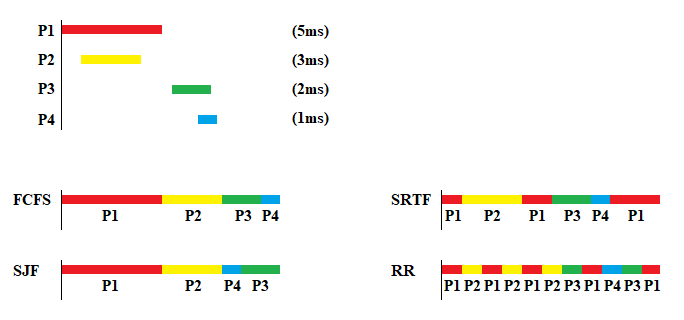
\includegraphics[width=\textwidth]{Sched.png}
\caption{Process Schedule}
\end{figure}

% Section 2
\section{Question 2}

\begin{verbbox}
Average waiting time: 
- FCFS	: W = 2.425 ms 
- SJF	: W = 2.175 ms 
- SRTF	: W = 1.675 ms 
- RR	: W = 2.675 ms 
\end{verbbox}

\fbox{
\theverbbox
}

% Section 3
\section{Question 3}

\begin{verbbox}
Average turnaround time:
* FCFS	: 
	T(P1) = 5 + 0 ms
	T(P2) = 3 + 4 ms
	T(P3) = 2 + 2.5 ms
	T(P4) = 1 + 3.2 ms
   -->  Average T = 5.175 ms
* SJF	: 
	T(P1) = 5 + 0 ms
	T(P2) = 3 + 4 ms
	T(P3) = 2 + 3.5 ms
	T(P4) = 1 + 1.2 ms
   -->  Average T = 4.925 ms
* SRTF	: 
	T(P1) = 5 + 6 ms
	T(P2) = 3 + 0 ms
	T(P3) = 2 + 0 ms
	T(P4) = 1 + 0.7 ms
   -->  Average T = 4.425 ms  
* SRTF	: 
	T(P1) = 5 + 6 ms
	T(P2) = 3 + 2 ms
	T(P3) = 2 + 1.5 ms
	T(P4) = 1 + 1.2 ms
   -->  Average T = 5.425 ms
\end{verbbox}

\fbox{
\theverbbox
}

\end{document}
